\documentclass[lang=cn,newtx,10pt,scheme=chinese]{elegantbook}

\title{模板 elegantbook.cls 使用示例}
\subtitle{为使用 \LaTeX{} 制作课程复习材料而生}

\author{kissdata}

% \date{2023/1/14}
% \version{1.0}

\extrainfo{感谢模板作者:Ethan Deng}

\setcounter{tocdepth}{3}

\logo{logo-blue.png}
\cover{cover.jpg}

\usepackage{pgfplots}
\usepackage{array}
\newcommand{\ccr}[1]{\makecell{{\color{#1}\rule{1cm}{1cm}}}}

% 修改标题页的橙色带
\definecolor{customcolor}{RGB}{32,178,170}
\colorlet{coverlinecolor}{customcolor}
\usepackage{cprotect}

\addbibresource[location=local]{reference.bib} % 参考文献

\begin{document}
	
	\maketitle % 封面

这是一个教学使用 tex 开源模块库 elegantbook 的案例。为什么用这玩意儿?\\
因为它在 2022 年底 “定型” 了,最终版本 v4.5。你可以在
\href{https://github.com/ElegantLaTeX/ElegantBook/releases}{github.com/ElegantLaTeX/ElegantBook} 下载。

	\frontmatter  % 目录链接
	\tableofcontents % 目录
	\mainmatter % 章节带序号,目录带页码



\chapter{文章整体布局框架}
	
	\section{去除无效努力}
	
	你的知识是课本的,整理的本质只是做个复读机,不要花精力维护封面、来源、出处这些。也不方便打印下来看。
	在目录前加一页代替封面,随便写点介绍更好。方法是,把文字内容写在 \lstinline|\frontmatter| 前面。
	具体参考 test1.tex。

	\section*{备注}
	
	加载图片方法。

\begin{lstlisting}[language=tex]
\begin{figure}[!htb]
	\centering
	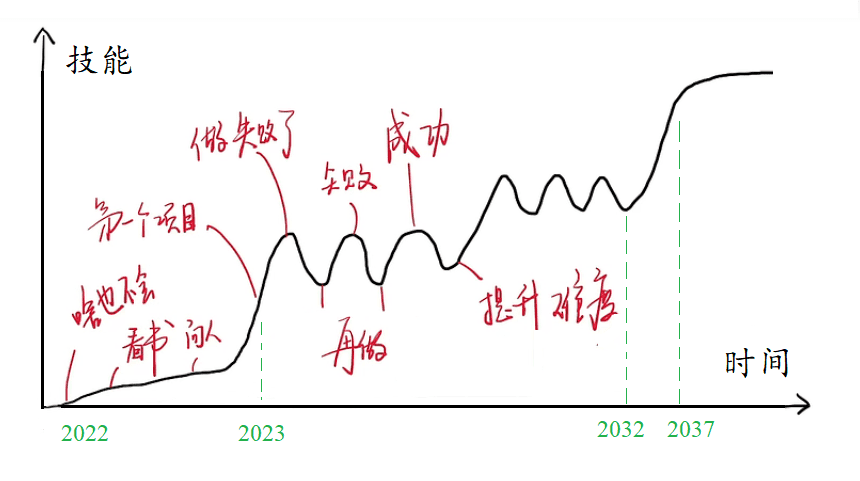
\includegraphics[width=0.9\textwidth]{life.png}
\end{figure}
\end{lstlisting}

图片在 image 目录,没有对应名字的图会报错。效果

	\begin{figure}[!htb]
		\centering
		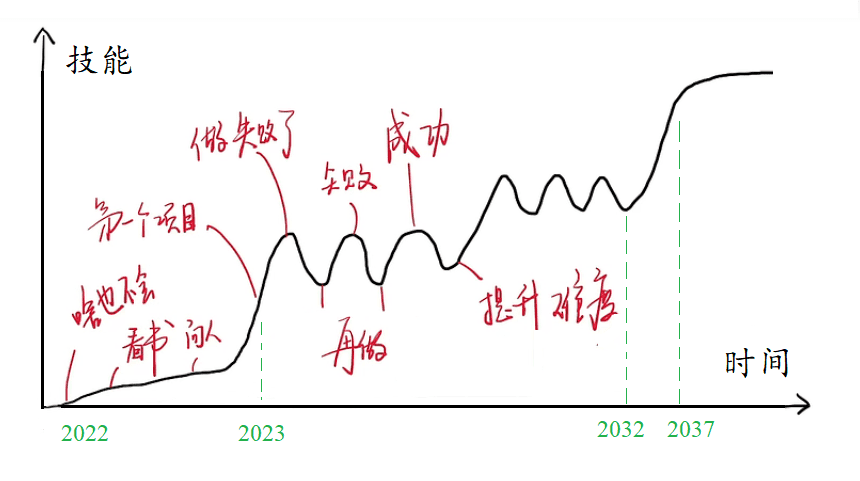
\includegraphics[width=0.9\textwidth]{life.png}
	\end{figure}



\chapter{数据图形问题}

这一章的功能跟 cls 文库库无关,是需要额外用 pgfplots 宏包。

一些数据产生的图片,不应该直接以图像的形式引入,虽然这样子更快。但好的话还是有 tex 代码画。
一是你找图得好久,有的还带水印,你再做裁剪、修改标注这些还要画精力;或者你自己用画图,拉框对下标也要好久;
二是如果数据要修改,图片还要整个重做。你用 tex 代码的图就容易了,而且 x 轴和 y 轴的文字数字都能直接复制。
当然,用 Matlab 或者 Python 导出pdf图也许更方便。

\section{画柱形图}

\begin{example}
	按照表数据生成一个研究近几年婚姻趋势的图(据说现在初婚年龄推迟到 28 岁)
\end{example}
效果

\pgfplotsset{width=9cm,compat=1.3}
\begin{tikzpicture}
\begin{axis}[ 
  x tick label style={/pgf/number format/1000 sep={}},
  ylabel=一季度登记数据(单位/万对),  
  enlargelimits=0.04, 
  legend style={at={(0.5, -0.12)}, anchor=north, legend columns=-1}, 
  ybar interval=0.8, ]
  \addplot 
    coordinates {(2019, 281.5) (2020, 155.7) (2021, 213.2) (2022, 210.7) (2023, 0)};
  \addplot 
    coordinates {(2019, 104.6) (2020, 61.2) (2021, 29.6) (2022, 51.4) (2023,0)};
  \legend{结婚, 离婚}
\end{axis}
\end{tikzpicture}

可以看到 2020 年很多人被疫情耽误了,没有结婚,不然应该是逐年递减。
近两年也是疫情,很多人没有离婚,2021 年疫情较紧的时候到了低谷。

从文档占空间看,有图和没图只差 5kB 左右。如果加一张这种图,压缩后也不止 5k吧。确实有它的好处,代码

\begin{lstlisting}
\pgfplotsset{width=9cm,compat=1.3}
\begin{tikzpicture}
	\begin{axis}[ 
		x tick label style={/pgf/number format/1000 sep={}},
		ylabel=一季度登记数据..., % y 轴说明
		enlargelimits=0.05, % 控制两个条的间距
		legend style={at={(0.5, -0.12)},  % 颜色注解距离 x 轴的位置
		anchor=north, legend columns=-1}, 
		ybar interval=1, ]
\addplot % 必须多写一个,最后一个数据不显示
	coordinates {(2019, 281.5) (2020, 155.7) (2021, 213.2) (2022, 210.7) (2023, 0)};
\addplot 
	coordinates {(2019, 104.6) (2020, 61.2) (2021, 29.6) (2022, 51.4) (2023,0)};
		\legend{结婚/万对, 离婚/万对}
	\end{axis}
\end{tikzpicture}
\end{lstlisting}


\chapter{还没想到}

已经够用了,以后用到再说

自动在上方加一横线

\datechange{2019/08/18}{版本 3.09 正式发布}

\begin{change}
  \item 新增目录选项 \lstinline{toc},可选项为单栏 \lstinline{onecol} 和双栏 \lstinline{twocol};
  \item 手动增加参考文献选项 \lstinline{cite},可选项为上标形式 \lstinline{super}。
  \item 引入 Note 模板中的 \lstinline{pad} 选项 \lstinline{device=pad}。
  \item 数学字体加入 \lstinline{mtpro2} 可选项 \lstinline{math=mtpro2},使用免费的 \lstinline{lite} 子集。
  \item 引入隐藏装饰图案选项 \lstinline{base},可选项有显示 \lstinline{show} 和隐藏 \lstinline{hide}。
  \item 新增定理模式 \lstinline{mode},可选项有简单模式 \lstinline{simple} 和炫彩模式 \lstinline{fancy}。
  \item 新增隐藏证明、答案等环境的选项 \lstinline{result=noanswer}。
\end{change}

\nocite{*}
\printbibliography[heading=bibintoc, title=\ebibname]

\appendix 

\chapter{没什么想说的}

	
\end{document}